\section{Methodology} \label{methodology}
This chapter describes how we use the theoretical framework to answer the research question. We share all the source files related to this study using a GitHub repository: \href{https://github.com/marioverhaeg/cs-thesis}{https://github.com/marioverhaeg/cs-thesis}.

\subsection{Research question} \label{meth_scope}
\subsubsection{Scope}
The results of this study should help decision-makers to move to evidence-based decision-making. This goal leads us to the main research question:
\begin{center}
\large\color{document}{\researchquestion} \\
\end{center}

We detect premature information using its completeness and reliability. We base the completeness of decision-relevant information on the availability of the required information and base the reliability of the decision-relevant information on the three metrics described in section \ref{tf_dmm} \nameref{tf_dmm}: reproducibility, consensus, and conflict. This decision meta-information allows us to calculate the information maturity-level. Section \ref{tf_dmm} \nameref{tf_dmm} also indicates that evidence-based decision-making depends on the quality of information. The information maturity-level measures the maturity, or quality, of information. Therefore, a higher information maturity-level contributes to evidence-based decision-making.

\paragraph{Ontology structure}
We use Semantic Web technologies to store the information that decision-makers use to justify their decisions. First, we need to know if we can create an ontology for evidence-based management. Next, we need to ensure that we can store the information completeness and reliability in this ontology and, based on the completeness and reliability, detect premature information. 

\begin{center}
\large\color{document}{\rqdsone} \\[0.3cm]
\large\color{document}{\rqdstwo} \\[0.3cm]
\large\color{document}{\rqdsthree} \\
\end{center}

\paragraph{Data presentation}
We transform the information completeness and reliability into the information maturity-level. Therefore, we need to define the information maturity-level explicitly. Once we know when a decision-maker is interested in the information maturity-level, we can find the right way to present the information maturity-level to the decision-maker. This presentation should make it easier for the decision-maker to understand the information maturity-level and decide if the decision-relevant information is mature enough to make the decision.

\begin{center}
\large\color{document}{\rqvisone} \\[0.3cm]
\large\color{document}{\rqvistwo} \\[0.3cm]
\large\color{document}{\rqvisthree} \\
\end{center}

\subsubsection{Out of scope}
The scope of this study is limited to verify if it is possible to detect premature information and to find the right way to present the information maturity-level to a decision-maker. The implementation in a production environment requires a different focus and scope. Premature information will stay premature until the decision-maker extends the ontology with new information or adjusts existing information. Extending the ontology with new information or adjusting existing information is not in the scope of this study. We also exclude an analysis of the scalability and performance of our proposals.

\subsection{Scientific approach} \label{meth_sa}
We answer the research questions using a case-study based on the reasoning and structure proposed by \cite{THE08}. The way we phrased the research question and the related sub-questions indicates a case study would be the most suitable method to answer these questions \parencite{BK06}. Figure \ref{fig:ds1} presents our conceptual approach. There is a natural iteration between the main contribution and the validation. We need to adjust a pattern if we question its suitability to solve the specified problem in the given context. When we adjust a pattern, the validation of the pattern in other contexts might require adjustments as well.

\begin{figure}[H]
\centering
  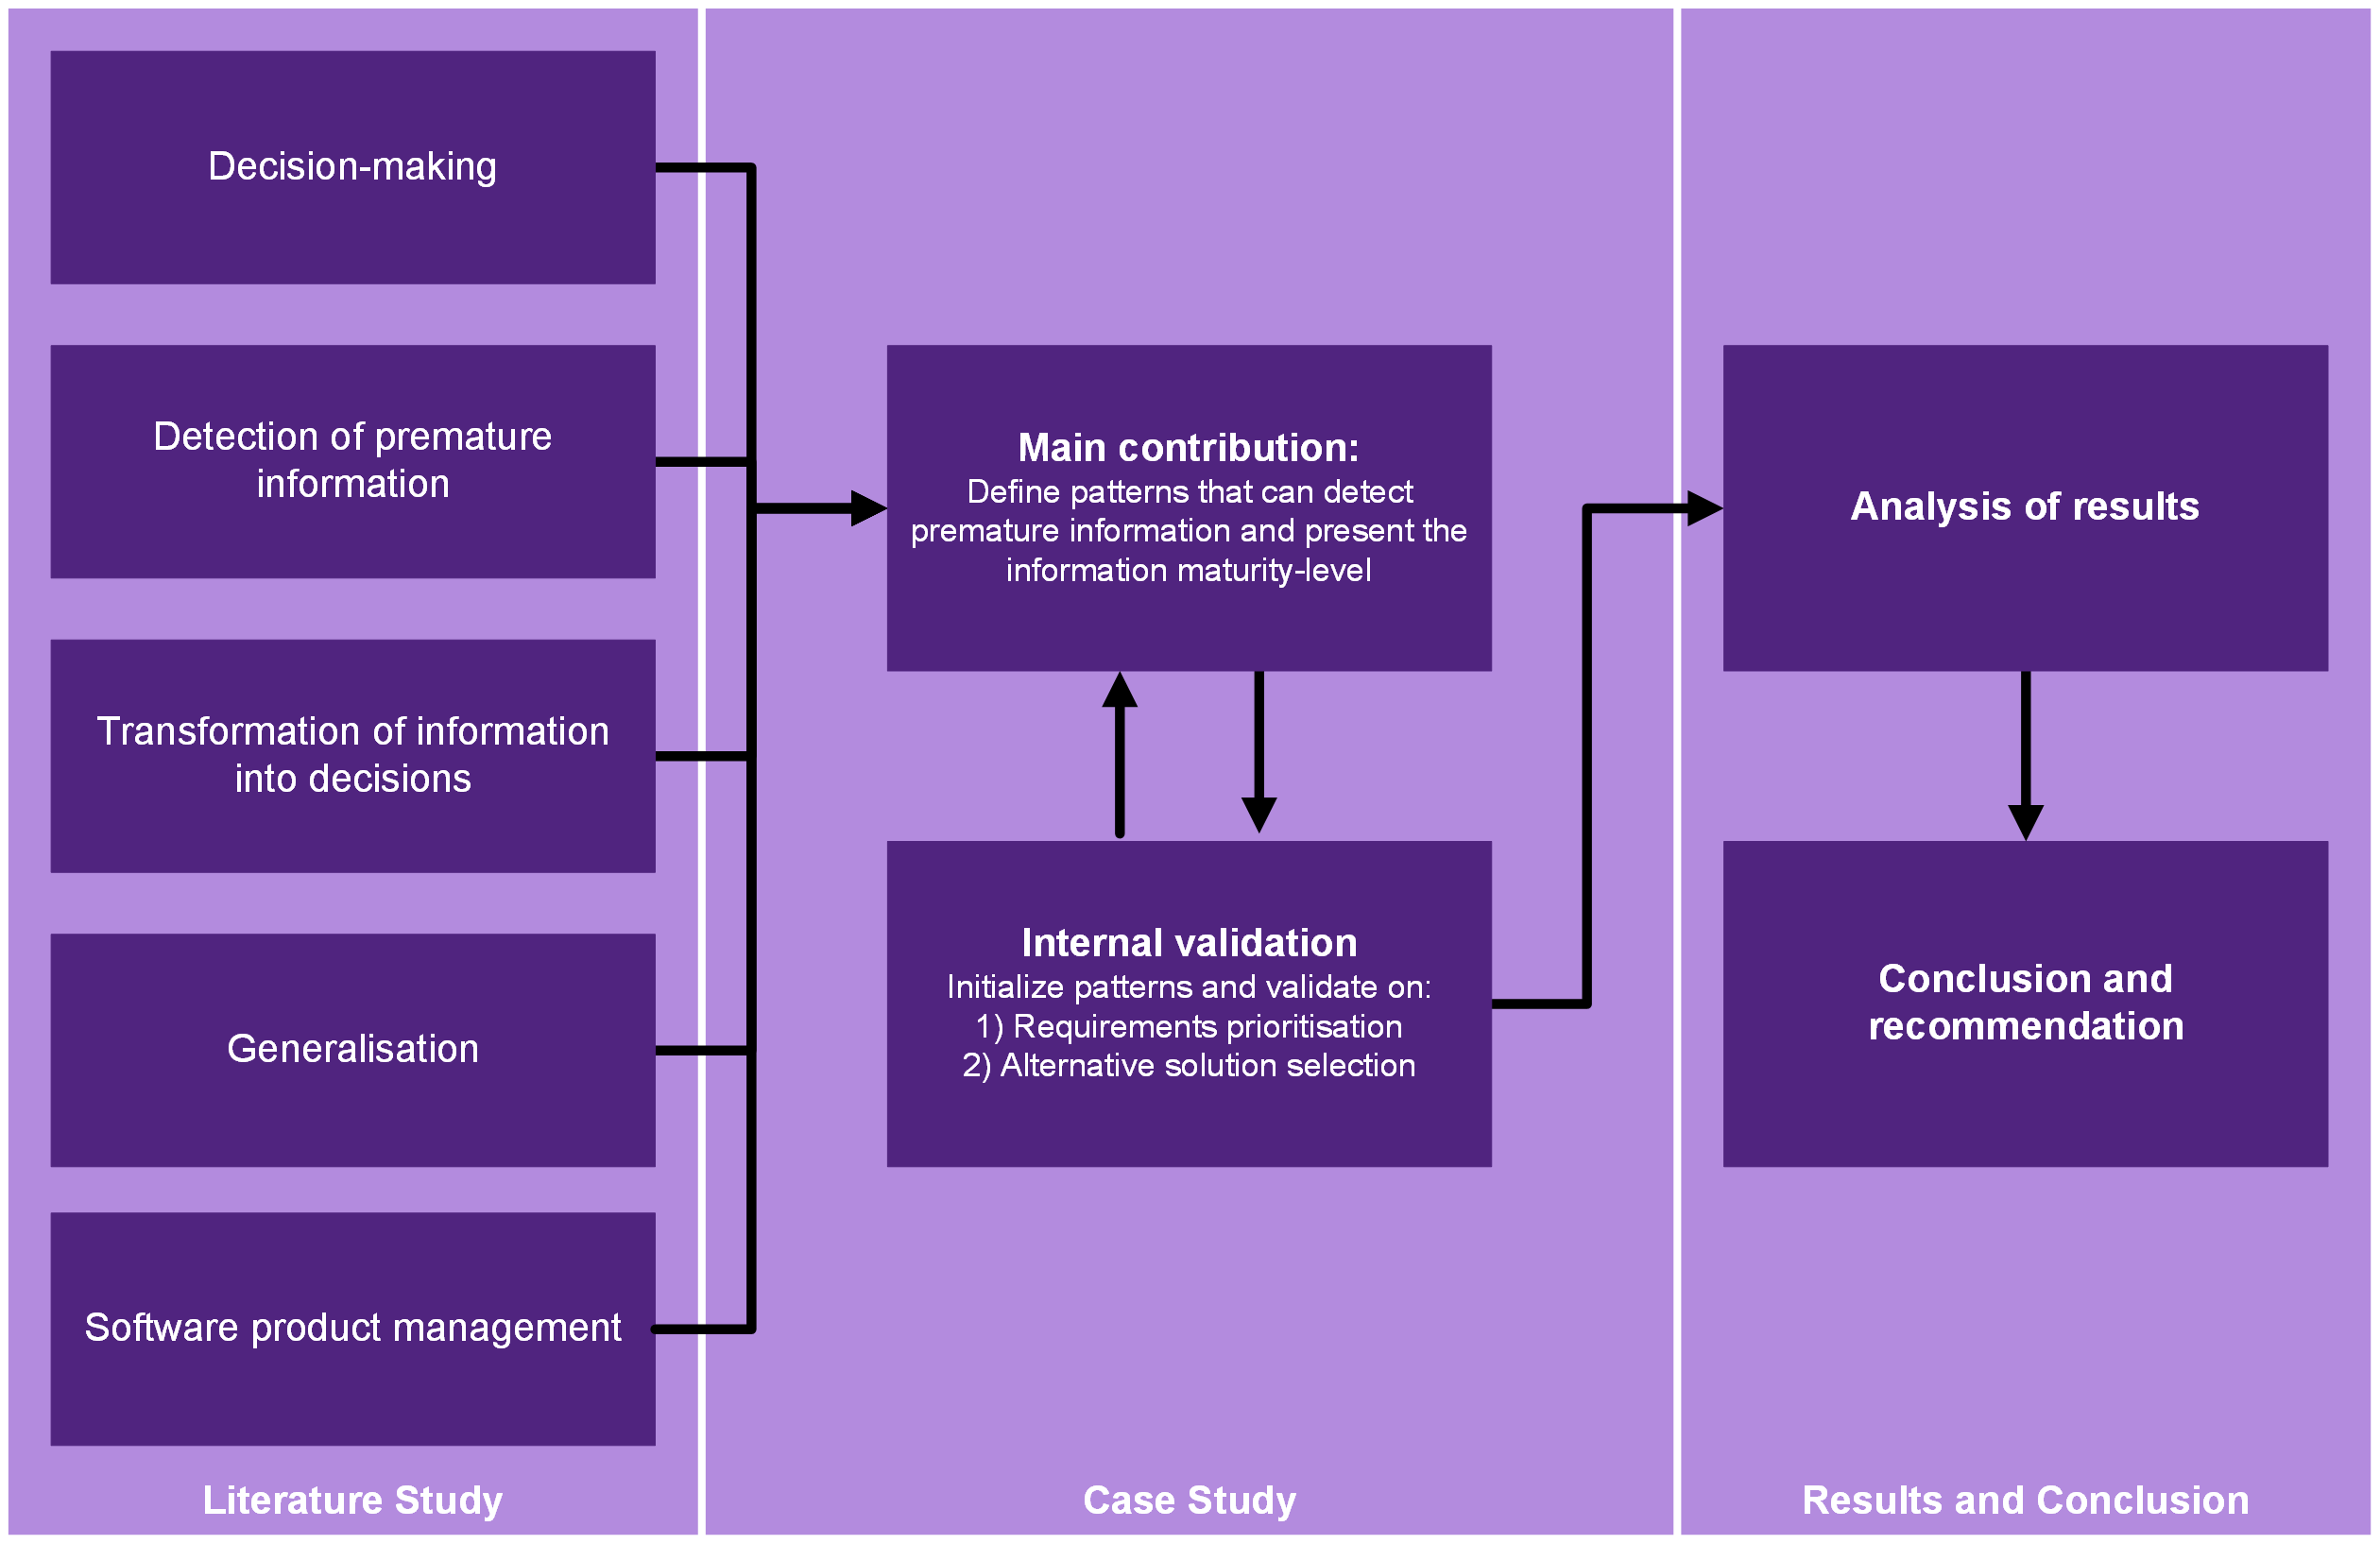
\includegraphics[width=16cm]{../../Images/03_Methodology/03_METH_Phases.png}
  \caption{The conceptual approach of this study, including the literature study, case study, and finalization phases. We re-use a structure proposed by \cite{THE08}.}
  \label{fig:ds1}
\end{figure}

A case study confirms the proposed concept works in a specific case. A pattern solves a general problem and should, therefore, be generally applicable. We validate the pattern on two scenarios to increase our confidence that the pattern is generally applicable. The first scenario validates the pattern and includes an extensive description of its reasoning and background. We reduce the level of detail in the second scenario to prevent repetition. We indicate when we leave out details and will refer to the approach we use in the first scenario. 

\subsection{Activities} \label{activities}
Table \ref{table:Tools} presents an overview of the tools described in this section\footnote{Prot\'eg\'e 5.5.0 uses rdflib 3.0.0. Rdflib 3.0.0 has an issue that prevents \emph{SPARQL COUNT DISTINCT} from working correctly (\href{https://github.com/RDFLib/rdflib/issues/404}{issue 404}). This issue is fixed in rdflib 5.0.0, but this version is not merged into Prot\'eg\'e yet. We ran into this issue on several occasions and worked around it by removing the COUNT and looking at the number of results of the SPARQL query.}.

\begin{table}[!htbp]
\centering
\caption{An overview of the tools used for this study.}
\begin{tabular}{| p{2cm} | p{1,5cm} | p{13,5cm} |}
\hline
\rowcolor{document}
\color{documentText}Name & \color{documentText}Version & \color{documentText}Description \\
\hline
\href{https://protege.stanford.edu/}{Prot\'eg\'e} & 5.5.0 & We use Prot\'eg\'e to create the base of the generic ontology design pattern, instantiating them manually and hosting the SHACL4P plugin. \\
\hdashline
\href{https://github.com/fekaputra/shacl-plugin}{SHACL4P} & 1.0.0 & We use SHACL4P for syntax checking and validating the constraints on instantiated generic ontology design patterns. \\
\hdashline
\href{https://github.com/spechub/Hets/tree/1899_gdol_parser}{HETS} & n/a & We use a branch of HETS ($1899\_gdol\_parser$) that adds support for Generic DOL, which is an extension of DOL. \\
\hline
\end{tabular}
\label{table:Tools}
\end{table}

\subsubsection{Ontology design patterns} \label{gen_meth}
We use generic ontology design patterns, described in section \ref{tf_odp} \nameref{tf_odp}, to define our ontologies formally. We use the open-source tool Prot\'eg\'e (the most widely used software for building and maintaining ontologies \parencite{ME08}) to create the base of the generic ontology design patterns and instantiate them manually. Additionally, we use HETS (the heterogeneous toolset) to validate the syntax of the generic ontology design patterns. At this moment it is not possible to use HETS to instantiate generic ontology design patterns into new ontologies or merge them into existing ontologies. We enter the ontologies into Prot\'eg\'e manually. 

\subsubsection{Detecting completeness and reliability}
We define a multi-layered model using Semantic Web technologies. This model can detect the completeness, consensus, conflict, and reproducibility of information or evidence. 

The first layer infers new information. Inferring information reduces the complexity of the constraints. We introduce a hierarchy of object properties and classes. When we connect two individuals using an object property in a hierarchy, the reasoner infers that the two individuals are connected by the parent of the used object property as well. Figure \ref{fig:ifop} presents an example of object property inferencing. In this case, we can define a single constraint for the abstraction layer, instead of defining multiple constraints that need to handle each case individually. Additionally, we further reduce the constraint complexity using the characteristics of an object property to infer chains of information and reduce the existing chains back into a single object property. Last, the reasoner infers class membership from the domain and range of an object property. Class membership ensures that the constraints are applied to the right information.

\begin{figure}[H]
\centering
  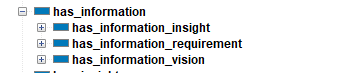
\includegraphics[width=8cm]{../../Images/03_Methodology/03_Inferring_Object_Properties.png}
  \caption{This example shows that the reasoner infers the object property $has\_information$ when the individual hosts the object property $has\_information\_insight$.}
  \label{fig:ifop}
\end{figure}

The second layer ensures the structural consistency of the ontology by defining that specific classes or object properties are disjoint. This definition makes the second layer especially useful to detect mistakes in the configuration of the inferencing rules.

The third layer validates the completeness and reliability of decision-relevant information:
\begin{enumerate}
\item We base the completeness on the existence of specific data- and object properties
\item Reproducibility equals the number of evidence sources used for decision-relevant information.
\item The consensus is equal to the number of agreements between different evidence sources.
\item The conflict is equal to the number of disagreements between different evidence sources.
\end{enumerate}

The decision design pattern defines Semantic Web constraints to detect incomplete information, the number of consensus and conflicts, and the number of evidence sources. We calculate the information maturity-level based on the number of violated constraints and the maximum number of constraints.

The Semantic Web provides two mechanisms to detect a violation of constraints: SPIN (SPARQL Rules) and SHACL. Compared to SHACL, SPIN never became a formal W3C standard, and the industry recognises SHACL as the successor of SPIN:
\begin{quote}\itshape
'SHACL supersedes SPIN in almost every respect. [...] Most importantly, SHACL is an official W3C Recommendation that makes it far more likely that other vendors will support it.' \parencite{WEB14}
\end{quote}

We select SHACL to detect the violation of constraints.

We use the Prot\'eg\'e plugin SHACL4P \parencite{SM25} to validate the SHACL shapes. SHACL4P allows us to define constraints and validates the ontology against those constraints. Figure \ref{fig:shacl-output} presents an example of the output of SHACL4P. 

\begin{figure}[H]
\centering
  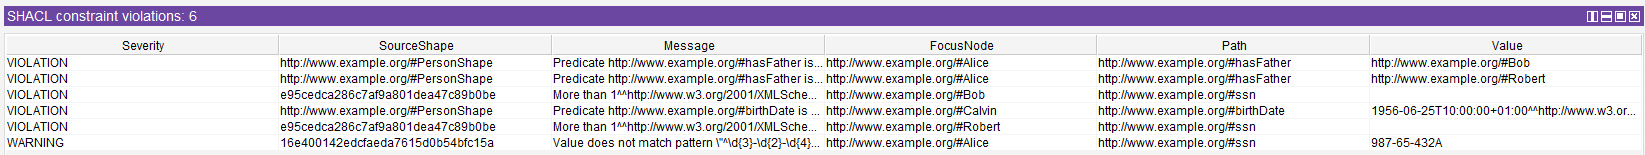
\includegraphics[width=17cm]{../../Images/SHACL4P_Example.png}
  \caption{An example of SHACL4P output showing constraint violations in Prot\'eg\'e.}
  \label{fig:shacl-output}
\end{figure}

\subsubsection{Constraint design patterns}
We cannot find an explicit definition of constraint design patterns. Therefore, we define the constraints in a way they are re-usable. We add parameters to the constraints when we need those constraints in the context of the ontology design patterns. When we use parameters, we need to instantiate the constraints manually. 

\subsubsection{Presentation design patterns} \label{meth_presentation}
We need to present the information maturity-level to the decision-maker. First, we extract information from the ontology to provide input to the functions that calculate the information maturity-level. Second, we select the right information presentation pattern based on the characteristics of the decision. We present the information maturity-level of the information using the selected pattern. 

We build mock-ups for the data presentation pattern using generic tools, for example, Microsoft PowerPoint.  

\subsection{Validation} \label{meth-validation}
We split the validation into reproducibility (how can the results of the study be reproduced?), internal validity (how can the results of the study be validated?), and external validity (how can de results of the study be applied to other cases?).

\subsubsection{Reproducibility}
We ensure the reproducibility of this study using scientific literature, documented interpretation of the literature, and where applicable, documented decisions. We use, when possible, open-source tools and use our GitHub repository (\href{https://github.com/marioverhaeg/cs-thesis}{https://github.com/marioverhaeg/cs-thesis}) to store the generic ontology design patterns, ontologies, constraints, and queries that we present in this document. Additionally, we also store the source of this document in the GitHub repository.

\subsubsection{Internal validity}
The goal of the decision design pattern is to motivate decision-makers to move from intuition-based decision-making to evidence-based decision-making by detecting premature information and presenting the information maturity-level. We also want domain experts to re-use the decision design pattern when they want their decision-makers to move from intuition-based decision-making to evidence-based decision-making. 

The internal validity addresses the validation of the research question based on the two scenarios described in section \ref{tf-val-rp} \nameref{tf-val-rp} and \ref{tf-val-as} \nameref{tf-val-as} of the theoretical framework:
\begin{enumerate}
\item \nameref{val-rp}
\item \nameref{val-as}
\end{enumerate}

\subsubsection{External validity}
The external validity addresses the validation of the research question based on the same problem in a different domain. This study focuses on a single domain (software product management). Therefore, external validation is outside of the scope of this study. We present the results of the study in a way it allows them to be applied to other domains as well.

\subsubsection{Sample data}
The goal of the sample data is to validate if the ontology design patterns we create are suitable to detect premature information and present the information maturity-level in requirements prioritisation and alternative solution selection. Unfortunately, it proved difficult to find sample data for requirements prioritisation and alternative solution selection. Therefore, we create sample data ourselves. We define multiple test scenarios. Each test scenario has its dedicated sample data and describes how this sample data contributes to the results of the scenario. 

Creating sample data also carries a risk: we might miss validating scenarios for which we have not created sample data. We try to mitigate this risk by separating the sample data for each test case and by creating small differences in the sample data we use for different test cases.